\documentclass[10pt,a4paper]{article}
\usepackage[utf8]{inputenc}
\usepackage[italian]{babel}
\usepackage{amsmath}
\usepackage{amsfonts}
\usepackage{amssymb}
\usepackage{graphicx}
\usepackage{siunitx}
\usepackage[left=2cm,right=2cm,top=2cm,bottom=2cm]{geometry}
\newcommand{\rem}[1]{[\emph{#1}]}
\newcommand{\exn}{\phantom{xxx}}
\usepackage[italian]{babel}
\usepackage[utf8]{inputenc}
\usepackage{siunitx}
\usepackage{graphicx}
\usepackage{xcolor}
\usepackage{amsfonts}
\usepackage{amsmath}
\usepackage{amsthm}
\usepackage{tikz}
\usepackage{pgfplots}
\usepackage{enumitem}
\usepackage{siunitx}
\usepackage{subcaption}
\date{\today}
\usetikzlibrary{shapes.geometric,calc,matrix,arrows,snakes,shapes,patterns}
\title{Esercitazione 10B: Caratteristiche porte logiche e semplici circuiti logici}
\author{Massimo Bilancioni, Alessandro Foligno}
\begin{document}	
\maketitle
	
	\section{Caratteristiche statiche}
	Si monta il circuito come in figura,, utilizzando resistenze con valori  $R\ped{2~nominale}=100\Omega $,~
	$R\ped{1~meas}\approx2.08\pm0.01 k \Omega$, l'ultima è la resistenza massima del potenziometro che ci permette di variare la tensione all'ingresso del componente (e quindi di mettere l'ingresso  H/L).\\
	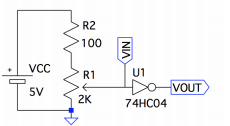
\includegraphics[scale=0.9]{Cattura.png}\centering
\\Si sono prese varie misure della tensione in ingresso/uscita,  ottenute variando la posizione del potenziometro; queste  sono riportate nella seguente tabella. Si è poi tracciato un grafico $V_{in}/V_{out}$ con i dati raccolti. \\
	
	\begin{center}
\begin{tabular}{|c|c|c|c|}
	\hline 
	$V_{in}(\si{\volt})$ & $\sigma(V_{in}) (\si{\volt})$ & $V_{out} (\si{\volt})$ & $\sigma(V_{out}) (\si{\volt})$ \\ 
	\hline 
	0.04&0.06&5.0&0.1\\ \hline
	0.28&0.05&5.0&0.1\\ \hline
	0.60&0.07&5.0&0.1\\ \hline
	1.00&0.06&4.9&0.1\\ \hline
	1.06&0.06&4.7&0.1\\ \hline
	1.18&0.06&3.88&0.08\\ \hline
	1.27&0.07&2.92&0.08\\ \hline
	1.40&0.08&1.50&0.08\\ \hline
	1.40&0.08&1.08&0.08\\ \hline
	1.48&0.08&0.10&0.08\\ \hline
	1.90&0.08&0.09&0.08\\ \hline
	2.40&0.08&0.08&0.07\\ \hline
\end{tabular} 
	\end{center}
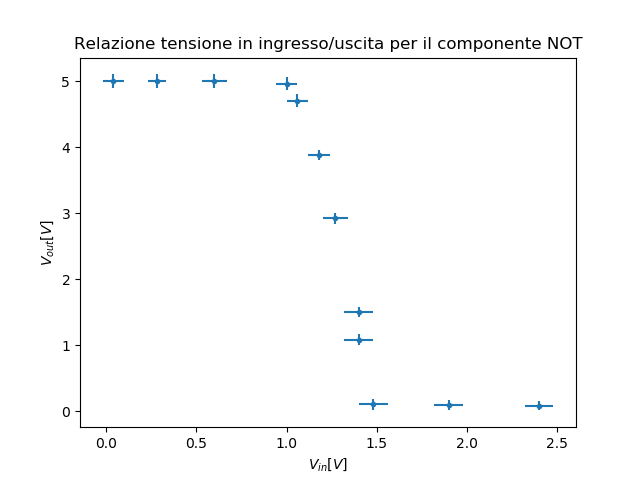
\includegraphics[scale=0.5]{gain.png}\centering
\\Come si può vedere, il comportamento del componente è quasi quello di una funzione a gradino, piuttosto piatta fino a un certo punto, e poi con una brusca variazione.
Osservando le coordinate degli "spigoli" del gradino, è possibile  stimare VIL, VOH  VIH, VOL e confrontare questi  con i valori riportati sul datasheet. In particolare le stime si  ottengono da i due punti subito prima e subito dopo la brusca variazione, che sono stati selezionati come punti limite per cui alzando/abbassando $V\ped{in}$ il segnale in uscita restava "costante".
\\

Si ottiene:
\begin{enumerate}
	\item $V_{IL}\approx0.9 V,~V_{IL~nominale}=0.8V$
	\item $V_{IH}		\approx 1.5V,~V_{IH~nominale}=2V$
	\item $V_{OL}\approx0.1V,~V_{OL~nominale}=0.5V$
	\item $V_{OH}\approx5V,~V_{OH~nominale}=2.7V$
\end{enumerate}
questi  risultati sono in linea con la formulazione "difensiva" del datasheet, infatti per i valori in ingresso il datasheet è meno elastico mentre per quelli in uscita dà delle condizione meno restrittive.

	\section{Caratteristiche dinamiche}

Abbiamo inviato in ingresso un'onda quadra con valore minimo $0 \si{\volt}$  e valore massimo circa $3 \si{\volt}$. Nelle Figure \ref{fig:phl},\ref{fig:plh}  compaiono l'ingresso (in arancio) e l'uscita (in blu) rispettivamente negli istanti in cui l'ingresso passa da basso ad alto e da alto a basso.
Nel primo caso misuriamo $t_{PHL}= (20\pm 2 )\si{\nano\second}$ nel secondo  misuriamo $t_{PLH} = (40\pm 4)\si{\nano \second}$.
Nel datasheet sono riportati i valori tipici: $t_{PHL}= 10 \,\si{\nano\second}$, $t_{PLH} = 9\,\si{\nano \second}$ e quello massimo $t_{PHL}^{MAX}= t_{PLH}^{MAX}= 15\, \si{\nano\second}$ che è quindi in disaccordo con il valore misurato. Ipotizziamo  che la discrepanza sia dovuta alla lentezza del generatore di onde quadre che impiega un certo tempo a passare da alto a basso.
Secondo le due Figure questo tempo è di circa $\sim 100 \, \si {\nano\second}$; a causa di questo, due fatti incidono sulla misura del tempo di propagazione: il primo è che per un intervallo dell'ordine delle decine di nanosecondi l'input non è né alto né basso ma compreso nella zona intermedia e questo può modificare la velocità con cui varia l'output; il secondo, secondo noi più rilevante, è che finchè $V\ped{in}$ non supera $V\ped{IL}$ nel primo caso (o scende sotto $V\ped{IH}$ nel secondo) l'uscita rimane invariata; il  tempo che  impiega l'input a raggiungere $V\ped{IL}$ (o  $V\ped{IH}$) non è una caratteristica del circuito integrato, ma produce un effetto di ritardo dello stesso ordine di grandezza (addirittura superiore, circa $25ns$) di quello che si vuole misurare dovuto esclusivamente all'integrato.Non è banale  compiere la misura escludendo quest'effetto, inoltre come si vede dalle Figure ciò causa anche asimmetria tra le due misure  $t_{PHL}$ e  $t_{PLH}$.
\begin{figure}[h]
			\centering
			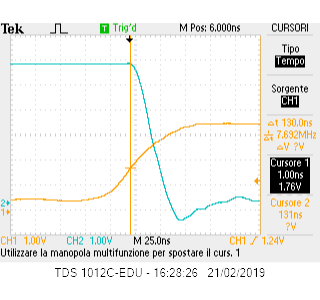
\includegraphics[scale=0.85]{schifo1}
			\caption{tempo di propagazione, misura di $t\ped{PHL}$}
			\label{fig:phl}
\end{figure}
\begin{figure}[h]
			\centering
			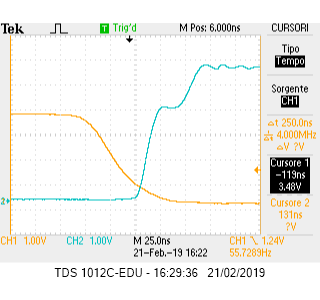
\includegraphics[scale=0.85]{schifo2}
			\caption{tempo di propagazione, misura di $t\ped{PLH}$}
			\label{fig:plh}
\end{figure}\clearpage
\section{Costruzione di circuiti logici elementari}
Si è verificato il comportamento della porta NAND tramite il led e l'interruttore con il circuito mostrato in figura \ref{NAND}.\\
\begin{figure}[h]\centering

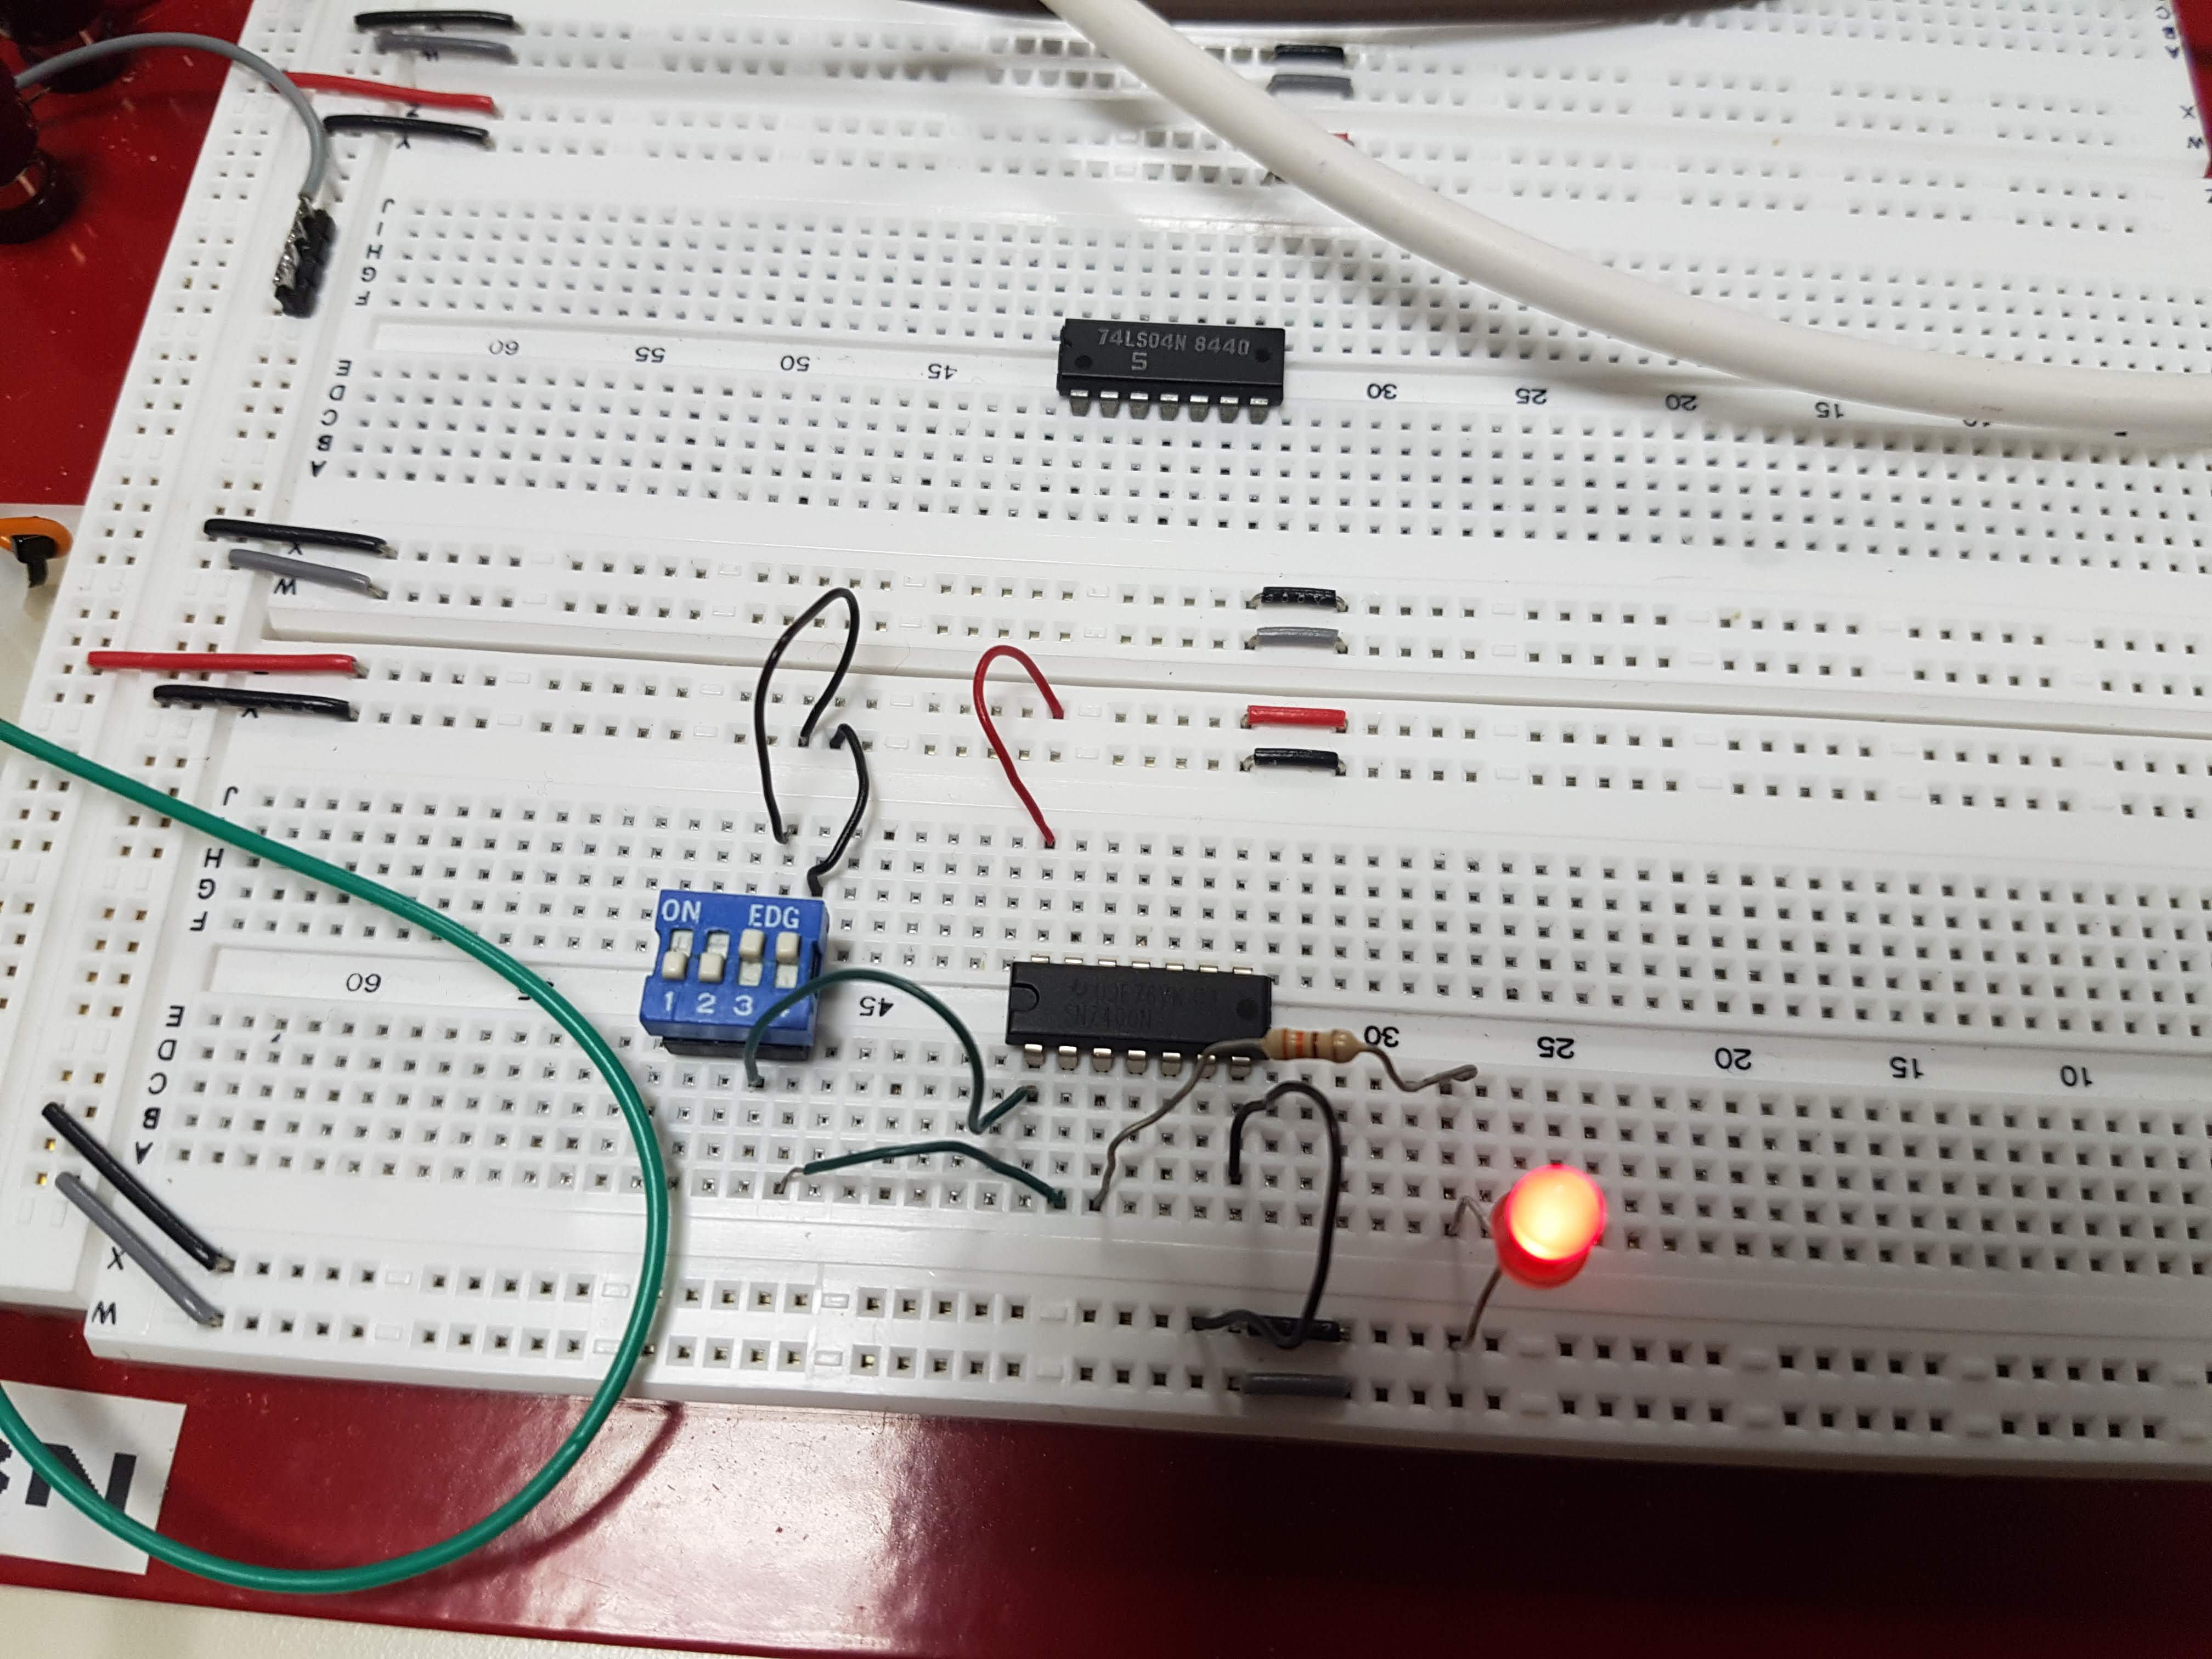
\includegraphics[scale=0.04]{20190221_164815.jpg}\label{NAND}
\caption{immagine del circuito realizzato per il NAND }
\end{figure}
Il circuito AND è stato costruito con due porte NAND secondo lo schema mostrato in Figura (\ref{fig:and}),il circuito realizzato è in Figura \ref{AND}.
\begin{figure}[h]\centering
	
	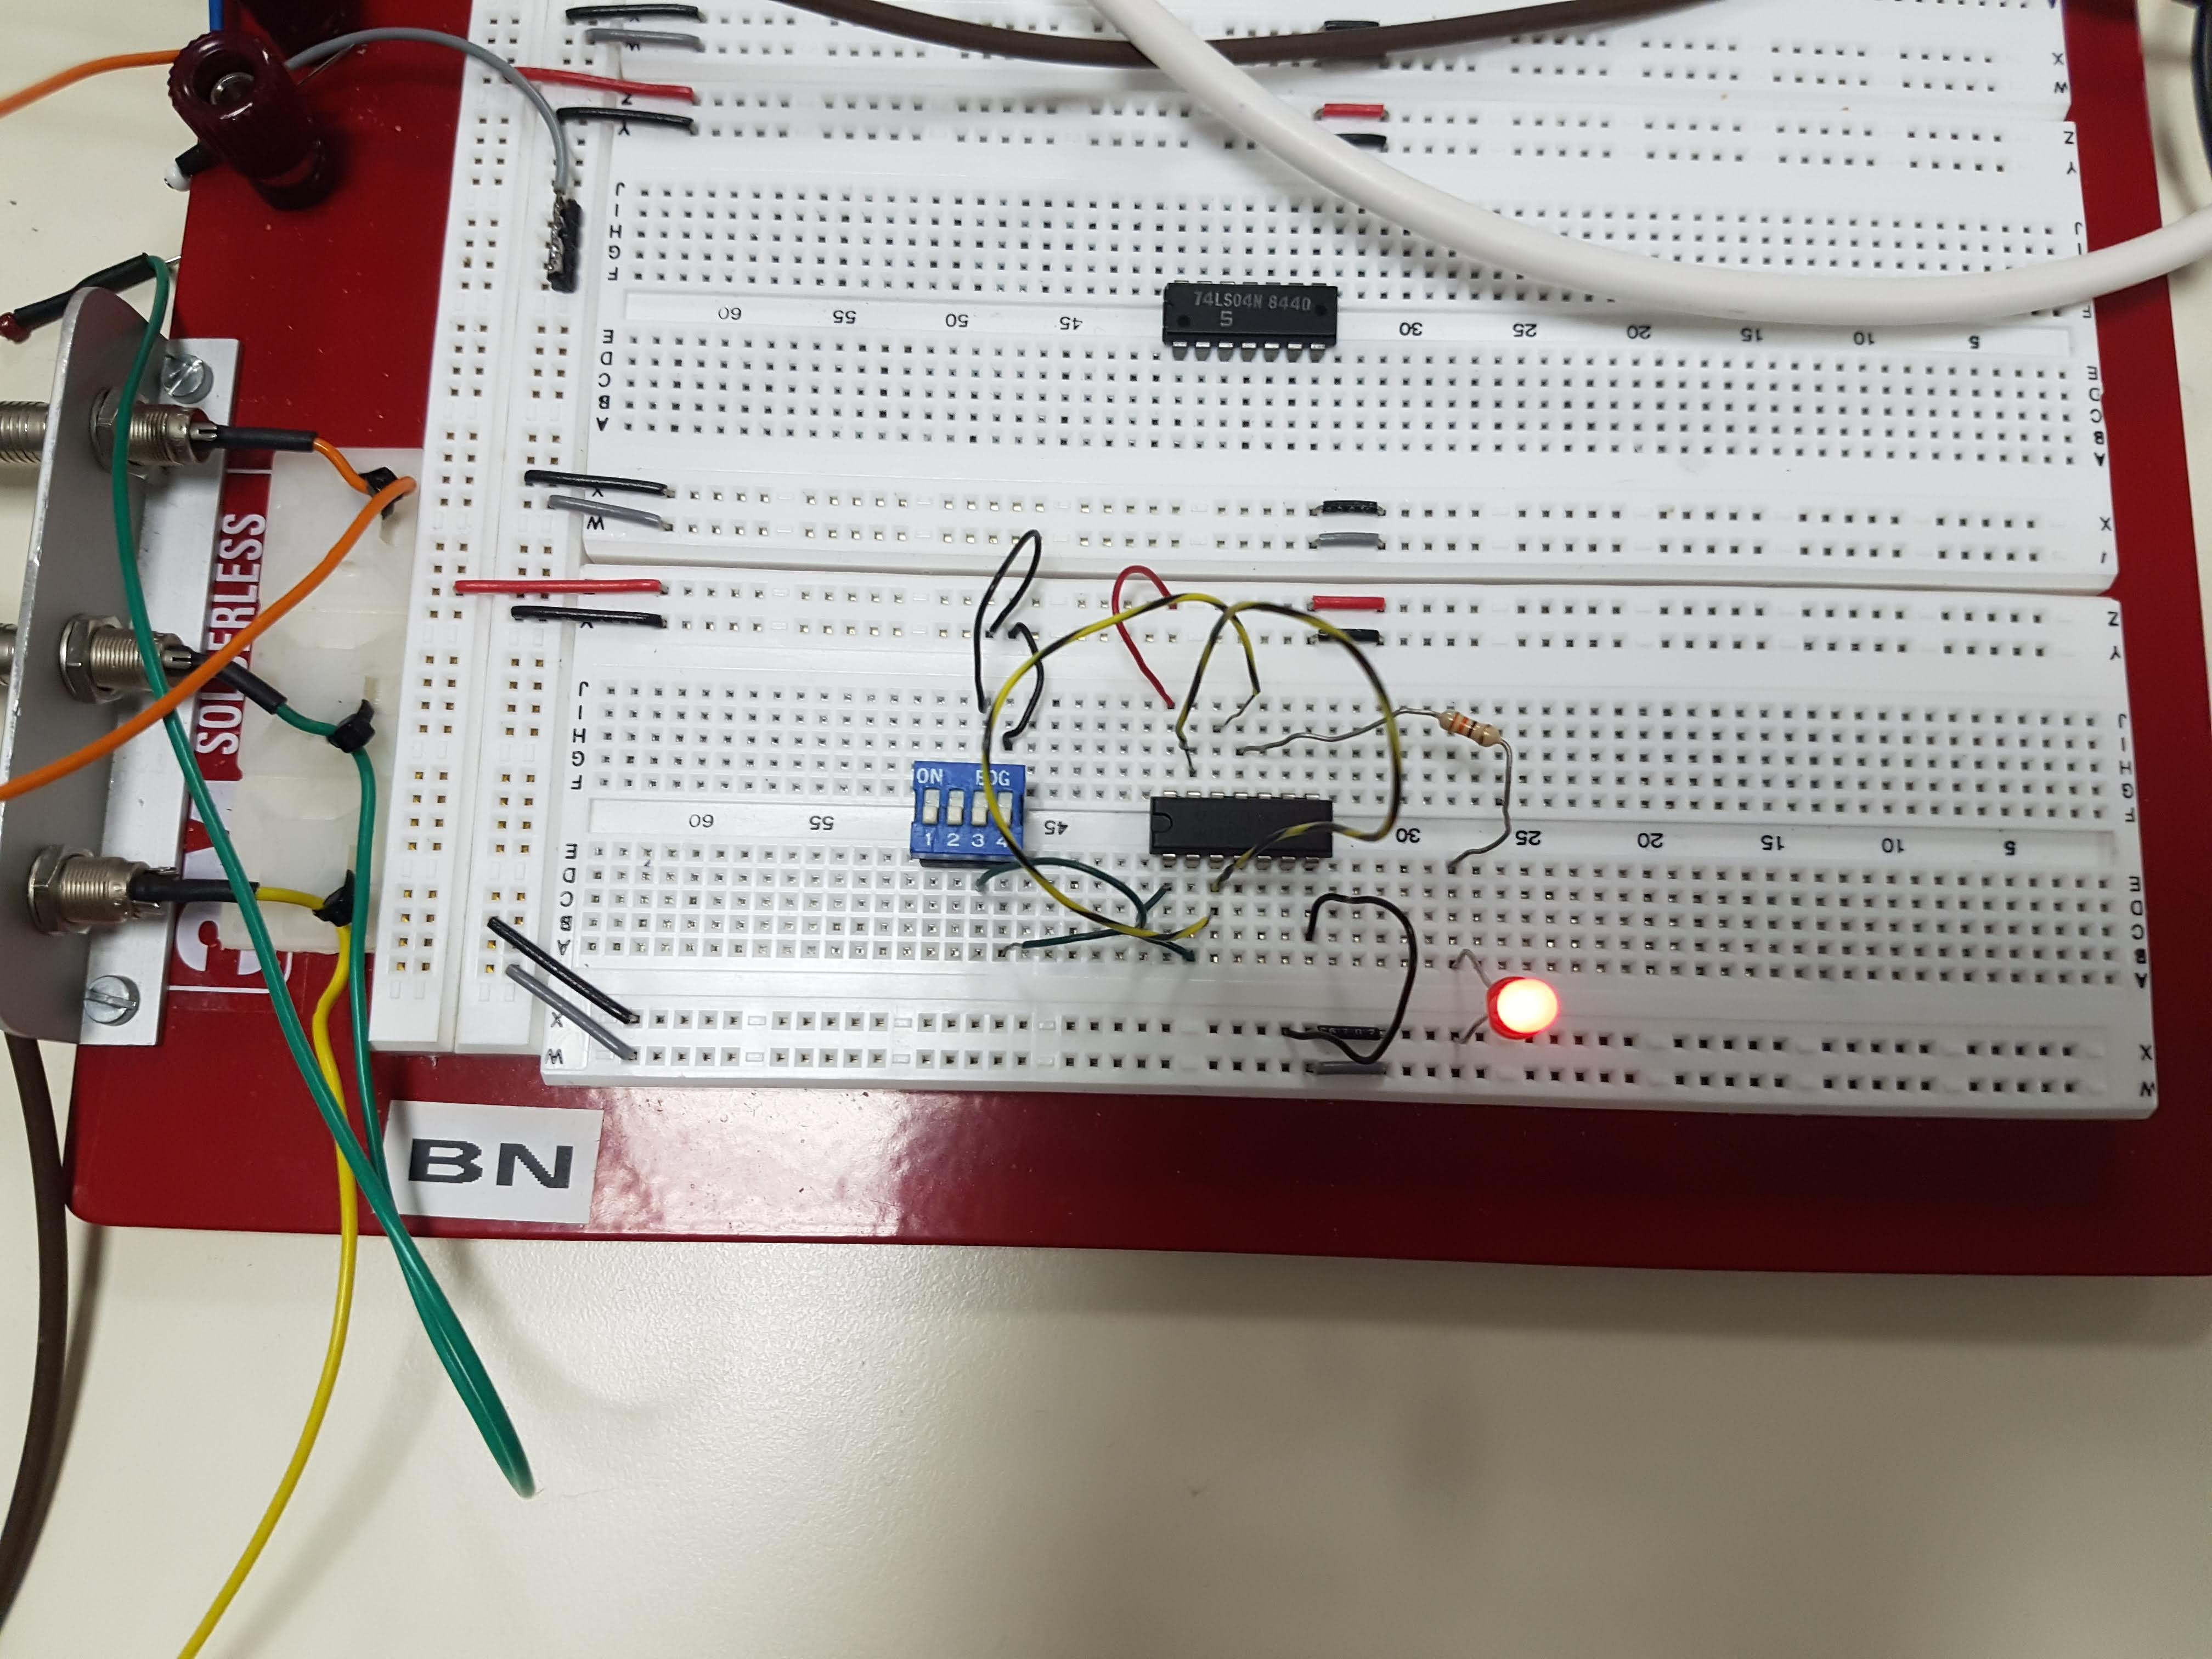
\includegraphics[scale=0.04]{20190221_165301.jpg}\label{AND}
	\caption{immagine del circuito AND }
\end{figure}\\

Per il circuito OR  si sono usate tre porte NAND, Figura (\ref{fig:or}), il risultato è riportato in figura \ref{OR}.
\begin{figure}[h]
	\centering
	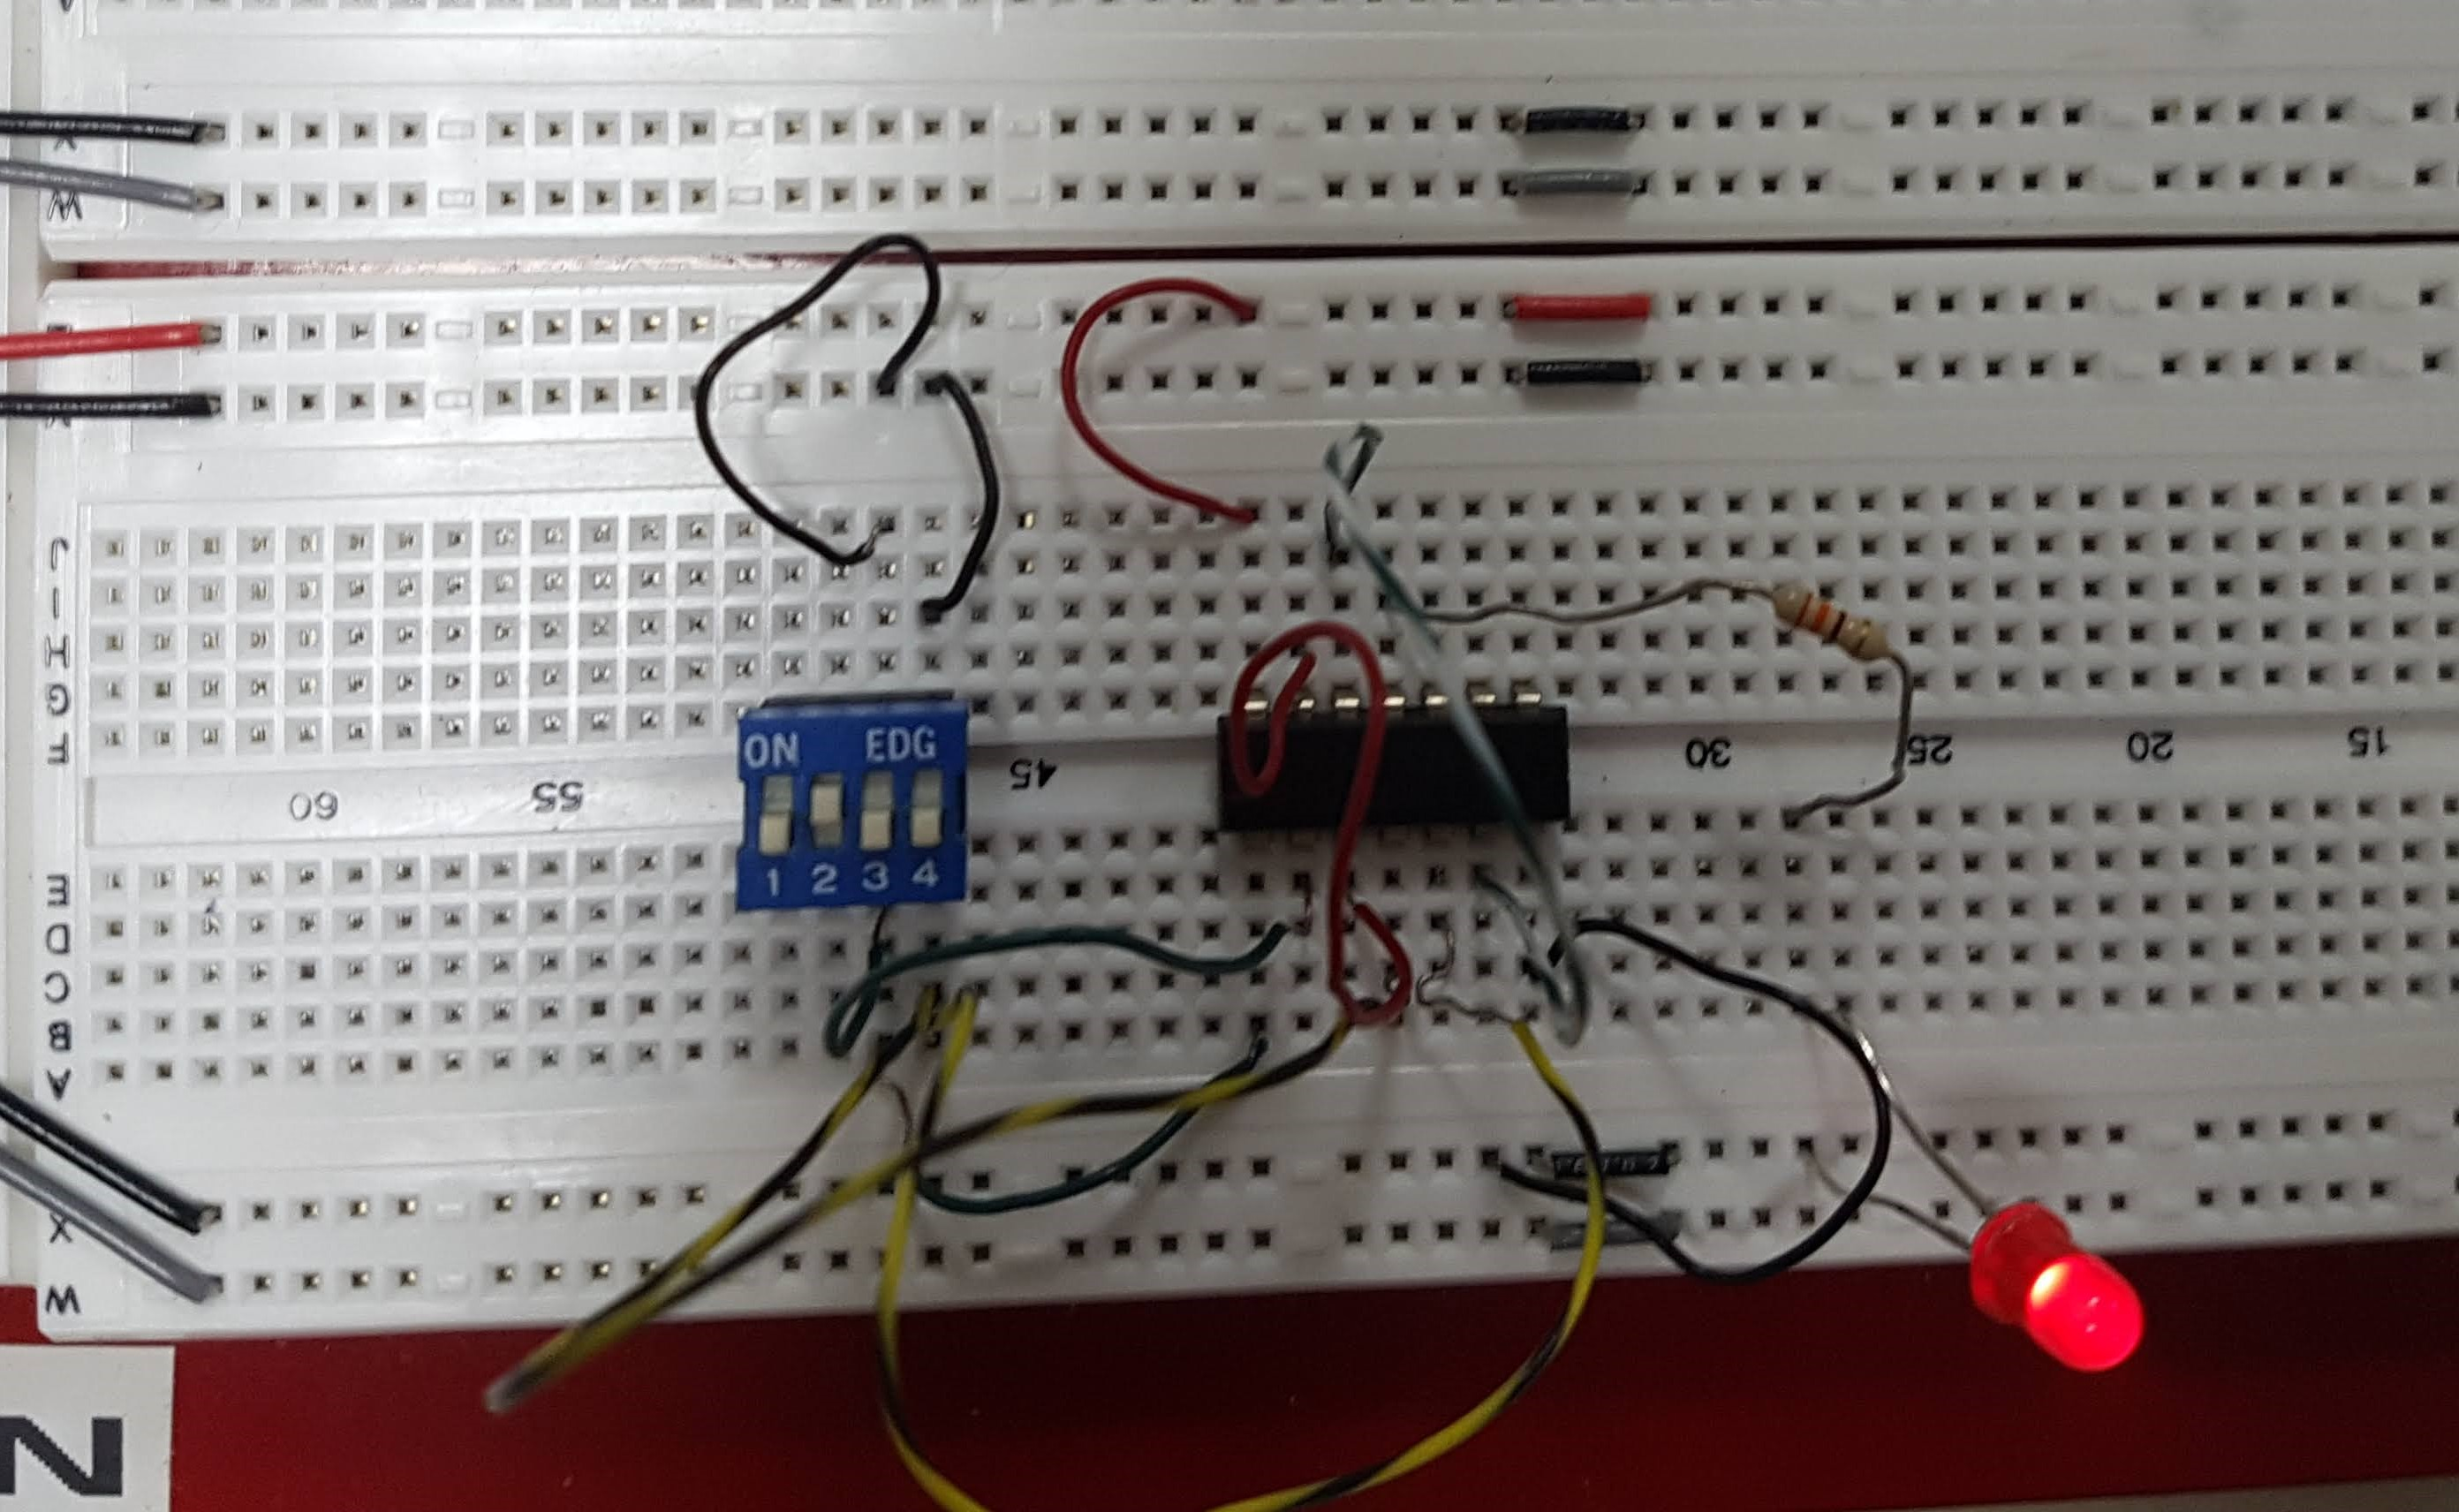
\includegraphics[scale=0.07]{20190221_170024.jpg}
	\caption{circuito OR realizzato}
	\label{OR}
\end{figure}
\\


Il circuito XOR  è stato realizzato con quattro porte NAND, Figura (\ref{fig:xor}),in Figura (\ref{XOR})  è riportata la realizzazione, (in realtà quello che è riportato è un sommatore a due bit, ma basta ignorare un output e un AND e resta uno XOR).

\begin{figure}[h]
			\centering
			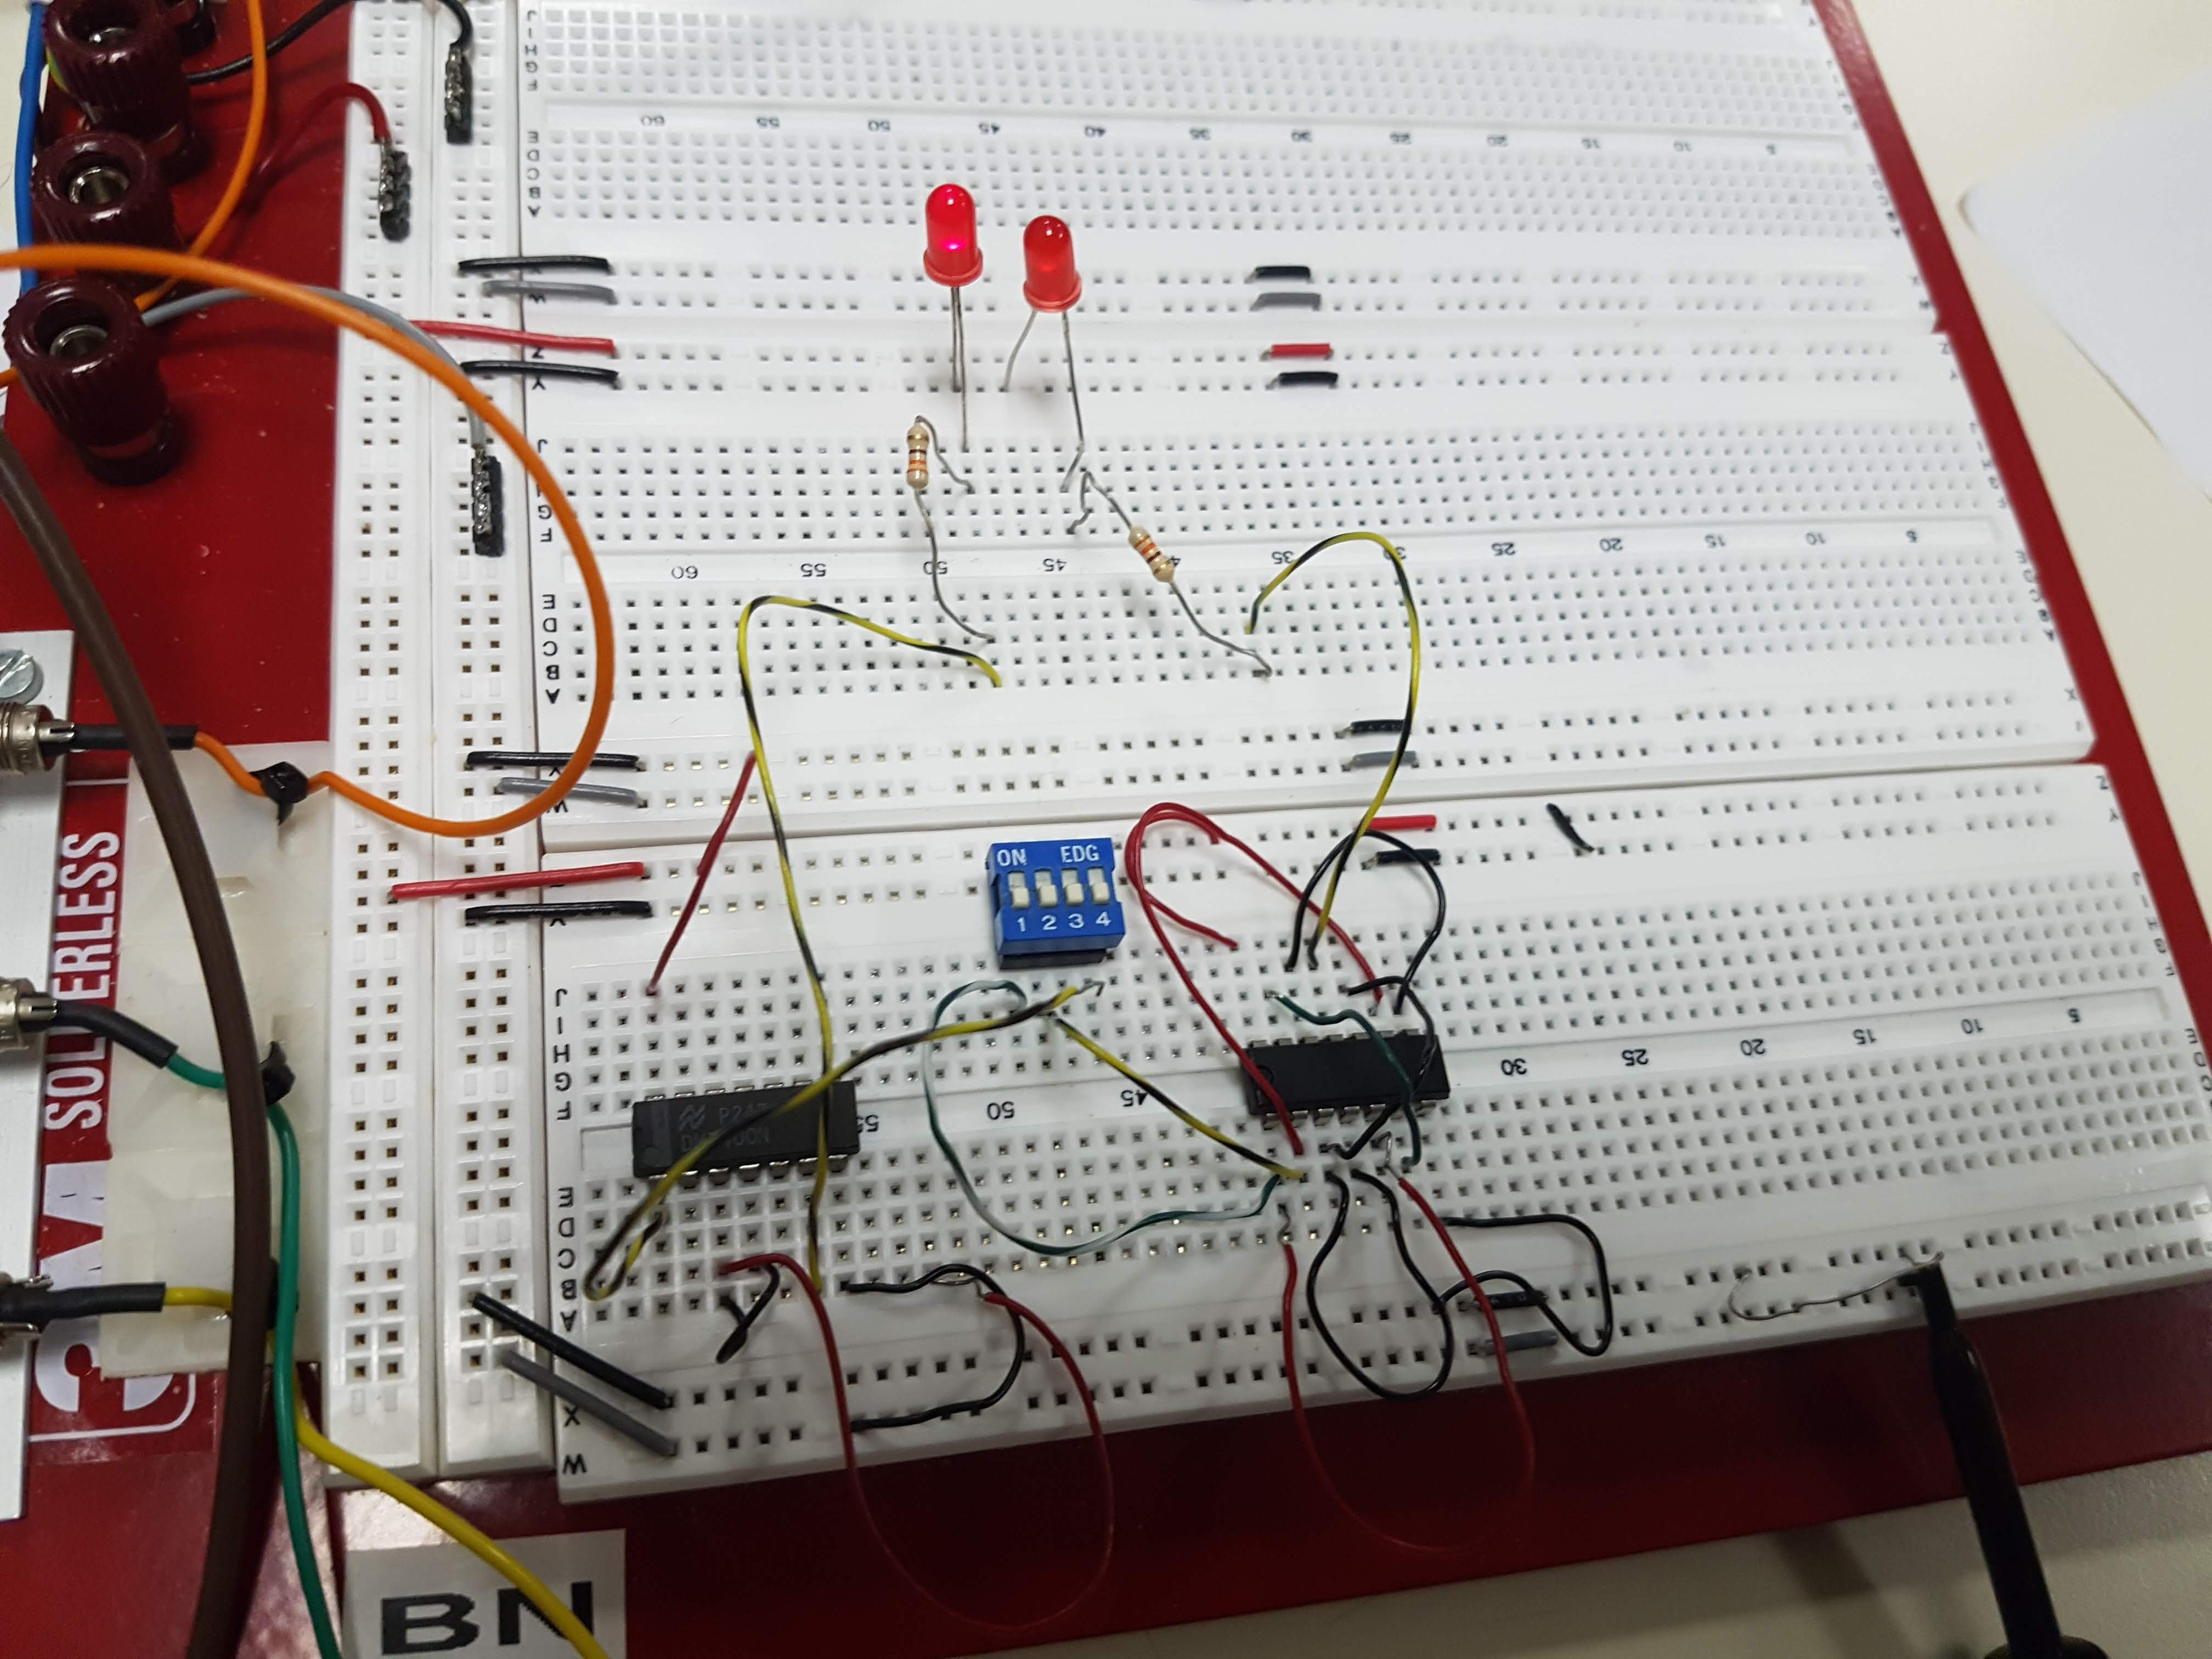
\includegraphics[scale=0.05]{20190221_180923.jpg}
			\caption{realizzazione sommatore a due bit (include lo XOR)}
			\label{XOR}
\end{figure}
\begin{figure}
	\centering
	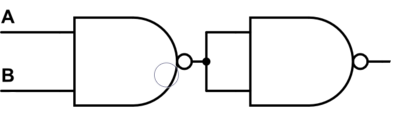
\includegraphics[scale=0.60]{and}
	\caption{schema porta AND}
	\label{fig:and}
\end{figure}
\begin{figure}
	\centering
	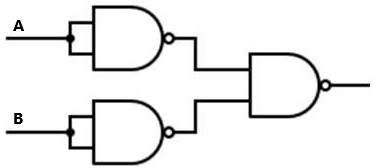
\includegraphics[scale=0.85]{or}
	\caption{schema porta OR}
	\label{fig:or}
\end{figure}
\begin{figure}
	\centering
	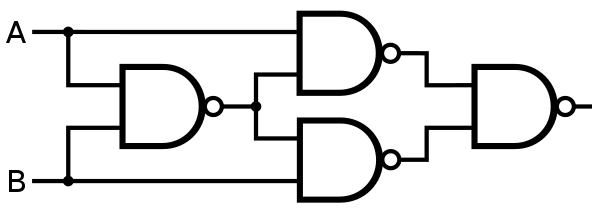
\includegraphics[scale=0.55]{xor}
	\caption{schema porta XOR}
	\label{fig:xor}
\end{figure}
Il sommatore a due bit è stato costruito con cinque porte NAND: una in meno rispetto alla somma AND $+$  XOR perchè una porta era in comune, Figura (\ref{fig:som}), guardare Figura \ref{XOR} per la realizzazione.
\begin{figure}
			\centering
			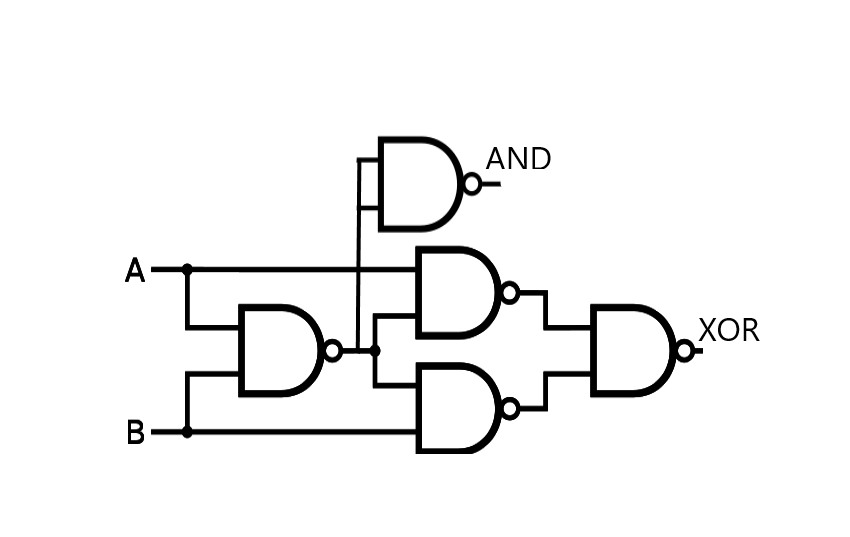
\includegraphics[scale=0.55]{sommatore}
			\caption{schema sommatore a due bit}
			\label{fig:som}
\end{figure}

Si sono verificati i comportamenti  previsti tramite l'accensione o meno del led  (due nel caso del sommatore a due bit) per tutte le configurazioni degli interruttori (due nel caso del sommatore a due bit).


\end{document}